% !TEX root = ../main.tex

\section{Introduction}
\begin{frame}
\frametitle{Introduction}
\end{frame}


\section{The Theta Neuron Model}
\begin{frame}
\frametitle{The Theta Neuron Model}
\tabitem SNIC bifurcation
\begin{figure}[H]
\minipage{0.33\linewidth}
\centering
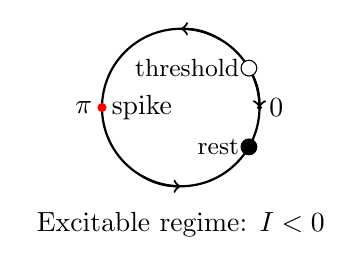
\begin{tikzpicture}
    \draw[thick] (0,0) circle [radius=1];
    \draw (0,-1.2) node[below]{Excitable regime: $I < 0$};
    \draw (-1,0) node[left]{$\pi$};
    \draw[fill=black, black] (1,0) circle [radius=0.025];
    \draw (1,0) node[right]{0};
    \draw[fill=red, red] (-1,0) circle [radius=0.05];
    \draw (-1,0) node[right]{spike};
    
    \draw[black, ->, thick] (0.866, 0.5)to[out=-60,in=90](1,0);
    \draw[fill=white, draw=black] (0.866,0.5) circle [radius=0.1];
    \draw (0.866,0.5) node[left]{\small{threshold}};
    
    \draw[fill=black, draw=black] (0.866,-0.5) circle [radius=0.1];
    \draw (0.866,-0.5) node[left]{\small{rest}};
    
    \draw[black, ->, thick] (0.5,0.866)to[out=150,in=0](0,1);
    \draw[black, ->, thick] (-0.5,-0.866)to[out=-30,in=180](0,-1);
\end{tikzpicture}
\endminipage
\minipage{0.33\linewidth}
\centering
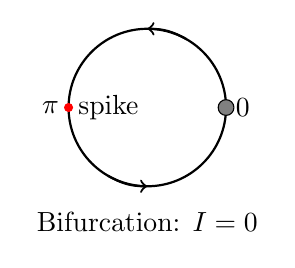
\begin{tikzpicture}
    \draw[thick] (0,0) circle [radius=1];
    \draw (0,-1.2) node[below]{Bifurcation: $I = 0$};
    \draw (1,0) node[right]{0};
    \draw[fill=red, red] (-1,0) circle [radius=0.05];
    \draw (-1,0) node[right]{spike};
    \draw (-1,0) node[left]{$\pi$};
    
    \draw[fill=gray, draw=black] (1,0) circle [radius=0.1];
    
    \draw[black, ->, thick] (0.5,0.866)to[out=150,in=0](0,1);
    \draw[black, ->, thick] (-0.5,-0.866)to[out=-30,in=180](0,-1);
\end{tikzpicture}
\endminipage
\minipage{0.33\linewidth}
\centering
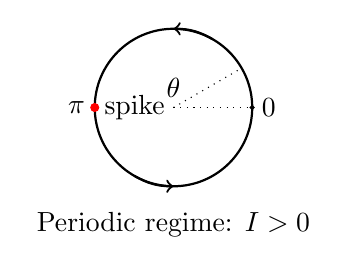
\begin{tikzpicture}
    \draw[thick] (0,0) circle [radius=1];
    \draw (0,-1.2) node[below]{Periodic regime: $I > 0$};
    \draw (-1,0) node[left]{$\pi$};
    \draw (1,0) node[right]{0};
    \draw[fill=black, black] (1,0) circle [radius=0.025];
    \draw[fill=red, red] (-1,0) circle [radius=0.05];
    \draw (-1,0) node[right]{spike};
    
    \draw[black, dotted] (0,0)to(1,0);
    \draw(0,0) node[above]{$\theta$};
    \draw[black, dotted] (0,0)to(0.866,0.5);
    
    \draw[black, ->, thick] (0.5,0.866)to[out=150,in=0](0,1);
    \draw[black, ->, thick] (-0.5,-0.866)to[out=-30,in=180](0,-1);
\end{tikzpicture}
\endminipage
\label{fig:thetaneuronbifurcationtikz}
\end{figure}

Features of the model
\begin{figure}[H]
\centering
\includegraphics[width = \textwidth]{../Figures/ThetaNeuronResponseToCurrent.pdf}
\label{fig:ThetaNeuronResponseToCurrent}
\end{figure}
\end{frame}

\begin{frame}
\frametitle{The Theta Neuron Model}
\begin{figure}[H]
\centering
\includegraphics[width = \textwidth]{../Figures/ThetaNeuronResponseToCurrent.pdf}
\label{fig:ThetaNeuronResponseToCurrent}
\end{figure}
\end{frame}



\section{Network Topologies}
\begin{frame}
\frametitle{Network Topologies}
\end{frame}


\section{Mean Field Reductions}
\begin{frame}
\frametitle{Mean Field Reductions}
\end{frame}

\section{\mywork Mean Field Reductions for undirected graphs} 
\begin{frame}
\frametitle{\mywork Mean Field Reductions for undirected graphs} 
\end{frame}


\section{Hebbian Learning and Synaptic Plasticity} 
\begin{frame}
\frametitle{Hebbian Learning and Synaptic Plasticity}
\end{frame}


\section{\mywork Emerging Network Topologies} 
\begin{frame}
\frametitle{\mywork Emerging Network Topologies}
\end{frame}


\section{Conclusion and Discussion} 
\begin{frame}
\frametitle{Conclusion and Discussion}
\end{frame}
